\documentclass[tikz,convert={outext=.svg,command=\unexpanded{pdf2svg \infile\space\outfile}},multi=false]{standalone}
\usepackage[utf8]{inputenc}
\usepackage{colortbl}



\begin{document}


\newcommand{\myface}[2]{\raisebox{-1.5mm}{\begin{tikzpicture}[scale=0.2]
\draw[fill=#1!10] (0, 0) ellipse (1cm and 1cm);
\draw[fill=blue!30] (-0.35, 0.4) ellipse (2mm and 2mm);
\draw[fill=blue!30] (0.35, 0.4) ellipse (2mm and 2mm);
\draw[red, line width=0.4mm] (-0.5, -0.4) edge[bend right=#2] (0.5, -0.4);
\end{tikzpicture}}}



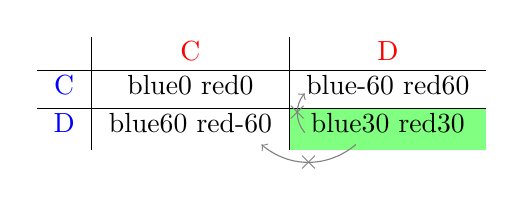
\begin{tikzpicture}
\node {\begin{tabular}{c|c|c}
 & \textcolor{red}{C} &  \textcolor{red}{D}
 \\
  \hline
 \textcolor{blue}{C} & \myface{blue}{0} \myface{red}{0} & \myface{blue}{-60} \myface{red}{60}   \\[0.5mm]% \includegraphics[width=5mm]{20franctrimetalrev.png} \\
  \hline
 \textcolor{blue}{D} & \myface{blue}{60} \myface{red}{-60}  & \cellcolor{green!50}\myface{blue}{30} \myface{red}{30}  \\[0.9mm]
\end{tabular}};
\draw[gray] (0.55, -0.5) edge[bend left=40, ->] node {$\times$} (0.55, 0);
\draw[gray] (1.2, -0.65) edge[bend left=40, ->] node {$\times$} (-0., -0.65);
 \end{tikzpicture}
 
 

\end{document}